

%%%%%%%%%%%%%%%%%%%%%%%% ADD CONTENT %%%%%%%%%%%%%%%%%%%%%%
\section{Introduction to programming}
\begin{frame}{\insertsectionnumber{ |} Command-line basics (*nix)}

\hspace*{-0.5cm}\textbf{Basic commands} \\
\vspace*{0.15cm}\begin{tabular}{p{0.75cm} p{6cm} p{3.5cm}}
\textbf{command} & \textbf{~~example} & \textbf{description} \\
ls & \Verb+ ls -ltrh + & \ul{l}i\ul{s}t directory contents (in long format, newest last) \\
cd & \Verb+ cd ../mydir/mysubdir + & \ul{c}hange \ul{d}irectory (up one level, down two) \\
rm & \Verb+ rm delete-this.txt and-all-these.* + & \ul{r}e\ul{m}ove file(s) \\
mv & \Verb+ mv rename-this.txt to-this.txt + & \ul{m}o\ul{v}e (rename) file(s) \\
mkdir & \Verb+ mkdir ./new-directory + & \ul{m}a\ul{k}e a new (empty) \ul{dir}ectory  \\
cp & \Verb+ cp this.txt ./new-dir/to-this.txt + & \ul{c}o\ul{p}y file (possibly to new location) \\
\end{tabular}


\vspace*{0.35cm}\hspace*{-0.5cm}\textbf{Linux c-line tools} \\
\vspace*{0.15cm}\begin{tabular}{p{0.75cm} p{6cm} p{3.5cm}}
\textbf{tool} & \textbf{~~example} & \textbf{description} \\
pwd & \Verb+ pwd + & Find out what your current \ul{p}ersonal \ul{w}orking \ul{d}irectory is \\
sed & \Verb+ sed -e `s/a/b/g'+ & \ul{s}tream \ul{ed}itor, swap `a' for `b' \\
awk & \Verb+ awk `\{print \$2, \$3\}'+ & print fields 2 \& 3 from file/stream \\
\end{tabular}

\vspace*{0.35cm}\hspace*{-0.5cm}\textbf{Other packages \& utilities} \\
\vspace*{0.15cm}\begin{tabular}{p{0.75cm} p{6cm} p{3.5cm}}
\textbf{package} & \textbf{~~example} & \textbf{description} \\
pdflatex & \Verb+ pdflatex myfile.tex + & compile \LaTeX ~document \\
git & \Verb+ git clone golledni/WinterSchool + & Make a local copy of a github repository \\
\end{tabular}


\end{frame}

%%%%%%%%%%%%%%%%%%%%%%%%

\begin{frame}[fragile]{\insertsectionnumber{ |} Simple (bash) shell scripting}



\begin{columns}
\column[c]{7.5cm}
\begin{itemize}

\begin{beamerboxesrounded}[lower=gray,shadow=true]{
\item We can combine many simple commands, tools, and utilities to achieve more complex tasks
}
\end{beamerboxesrounded}
\end{itemize}
\end{columns}

\vspace*{1cm}\begin{lstlisting}
pwd
/home/golledni/MEGA/Work/AntSciPlat/WinterSchool

pwd | sed -e `s/\// /g' | awk `{print "Today my",$1,"is the",$NF}'
Today my home is the WinterSchool
\end{lstlisting}


\begin{beamerboxesrounded}[lower=gray,shadow=true]{
\vspace*{0.5cm}
}
\end{beamerboxesrounded}

\end{frame}


%%%%%%%%%%%%%%%%%%%%%%%%

\begin{frame}{\insertsectionnumber{ |} Simple (bash) shell scripting}

\begin{columns}
\column[c]{7.5cm}
\begin{itemize}

\begin{beamerboxesrounded}[lower=gray,shadow=true]{
\item But to do anything more complex than simple pipes we probably want to write a script file to contain our sequence of commands:
}
\end{beamerboxesrounded}

\end{itemize}
\end{columns}

\vspace*{0.5cm}\centering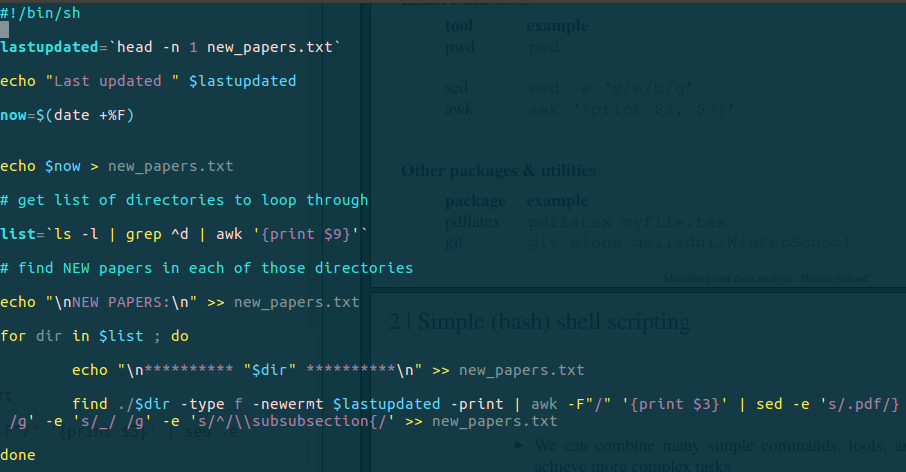
\includegraphics[width=10cm]{./images/sh-script.png}\\



\end{frame}


%%%%%%%%%%%%%%%%%%%%%%%%

\begin{frame}{\insertsectionnumber{ |} Control structures}

\begin{columns}
\column[c]{4cm}
\begin{itemize}

\begin{beamerboxesrounded}[lower=gray,shadow=true]{
\item Often we want to apply a test, or series of tests, to the data we're processing, and do different things with the data depending of the results of those tests
\item Control structures are what help us achieve this, and are fundamental to all languages
\item The two most common generic structures are 
\begin{itemize}
\item \Verb+if+ statements, and
\item \Verb+for+ or \Verb+do+ loops 
\end{itemize}}
\end{beamerboxesrounded}

\end{itemize}

\column[c]{5.5cm}

\Verb+if+ statement:
\begin{beamerboxesrounded}[lower=gray,shadow=true]{
\Verb+ i=0 +              \\
\Verb+ if [ \$i -ge 1 ] + \\
\Verb+ then +             \\
\Verb+ ~~~echo "i = \$i" +\\
\Verb+ else +             \\
\Verb+ ~~~echo "i < 1" +  \\
\Verb+ fi +
}
\end{beamerboxesrounded}


\vspace*{1cm}\Verb+do+ loop:
\begin{beamerboxesrounded}[lower=gray,shadow=true]{
\Verb+ i=0 +              \\
\Verb+ imax=10 +              \\
\Verb+ while [ \$i -le imax ] ; do + \\
\Verb+ ~~~echo "i = \$i" +\\
\Verb! ~~~i=`expr \$i + 1` !  \\
\Verb+ done +
}
\end{beamerboxesrounded}


\end{columns}




\end{frame}



%%%%%%%%%%%%%%%%%%%%%%%%

\begin{frame}{\insertsectionnumber{ |} ``Hello, World!''}

\begin{columns}

\column[c]{5cm}

Bash:
\begin{beamerboxesrounded}[lower=gray,shadow=true]{
\Verb+ \#!/bin/sh + \\
\Verb+  + \\
\Verb+ echo "Hello, World!" +             
}
\end{beamerboxesrounded}


\vspace*{0.5cm} Python:
\begin{beamerboxesrounded}[lower=gray,shadow=true]{
\Verb+ \#!/usr/bin/env Python +   \\
\Verb+  +              \\
\Verb+ print "Hello, World!" + 
}
\end{beamerboxesrounded}


\vspace*{0.5cm} Julia:
\begin{beamerboxesrounded}[lower=gray,shadow=true]{
\Verb+ \#!/usr/bin/env Julia + \\
\Verb+  +              \\
\Verb+ print("Hello, World!") + 
}
\end{beamerboxesrounded}

\column[c]{5.5cm}

Fortran 90:
\begin{beamerboxesrounded}[lower=gray,shadow=true]{
\Verb+ PROGRAM HELLOWORLD +  \\
\Verb+ + \\
\Verb+ ~~~IMPLICIT NONE + \\
\Verb+ ~~~print *, 'Hello, World!' + \\
\Verb+ + \\
\Verb+ END + 
}
\end{beamerboxesrounded}


\vspace*{0.5cm} C++:
\begin{beamerboxesrounded}[lower=gray,shadow=true]{
\Verb+ \#include <iostream> +   \\
\Verb+                              +\\
\Verb+ int main() \{ +              \\
\Verb+ ~~~std::cout << "Hello, World!"; + \\
\Verb+ ~~~return 0; + \\
\Verb+ \} + 
}
\end{beamerboxesrounded}


\end{columns}

\end{frame}



%%%%%%%%%%%%%%%%%%%%%%%%


\begin{frame}{\insertsectionnumber{ |} Interpreted vs. compiled languages}



\begin{itemize}

\item \underline{Compiled languages} require a \emph{compiler} to convert user code into machine code
\item Typically they create a platform-dependent binary (executable) file
\item If the code doesn't change, the binary can be run again and again
\item Once compiled, programs using these languages are typically very fast to run

\vspace*{1cm}\item \underline{Interpreted languages} read and execute user code line-by-line
\item No separate compilation step is required, so programs are platform-\emph{in}dependent
\item But, interpretation has to happen every time the code is run
\item As a result, this kind of code is typically slow to run

\end{itemize}

\end{frame}


%%%%%%%%%%%%%%%%%%%%%%%%


\begin{frame}{\insertsectionnumber{ |} Just-in-time compilers}


\begin{columns}

\column[c]{4cm}

\begin{beamerboxesrounded}[lower=gray,shadow=true]{

Just-in-time (JIT) compilation: \\

\begin{itemize}

\item Some modern languages like \textbf{Julia} use the JIT (or dynamic compilation) approach
\item With JIT, compilation of relevant code occurs \underline{at runtime}
\item If same packages / modules are called in subsequent runs, no re-compilation is necessary
\item This approach combines the best aspects of interpreted and compiled languages
\end{itemize}
}
\end{beamerboxesrounded}


\column[c]{6cm}


\includegraphics[width=6cm]{images/julia_web.png}

\end{columns}

\end{frame}


%%%%%%%%%%%%%%%%%%%%%%%%


\begin{frame}{\insertsectionnumber{ |} Speeding things up with functions}


\begin{columns}

\column[c]{6.5cm}
\begin{itemize}

\item A function is a block of code that does a specific job
\item Because it sits outside the main code sequence it only needs to be compiled and optimized once, even if it is used repeatedly
\item This makes your code faster :-)

\end{itemize}

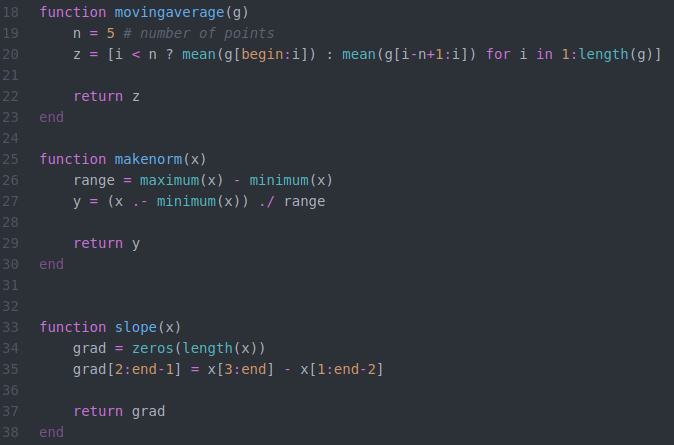
\includegraphics[width=6cm]{images/functions1.png}


\column[c]{5cm}

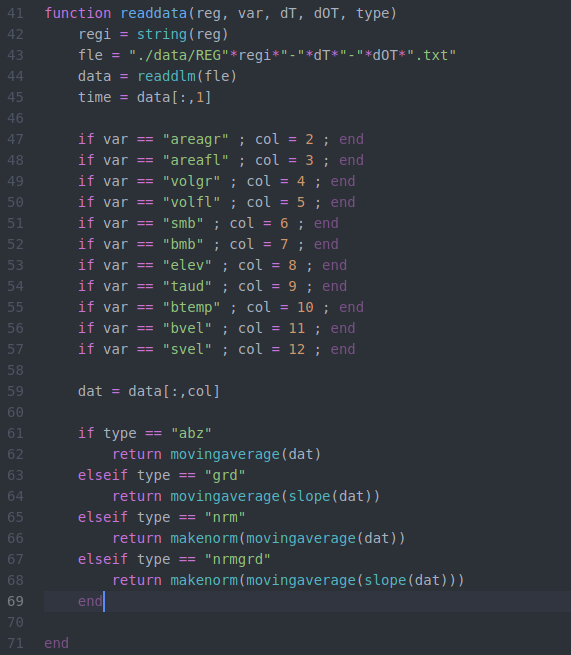
\includegraphics[width=5.25cm]{images/functions2.png}

\end{columns}

\end{frame}



%%%%%%%%%%%%%%%%%%%%%%%%


\begin{frame}{\insertsectionnumber{ |} Fundamentals of numerical modelling}


\begin{columns}

\column[c]{6cm}

\begin{beamerboxesrounded}[lower=gray,shadow=true]{
\begin{itemize}
\item Usually, a numerical model consists of a set of calculations that are repeated
\item Typically, each repetition of the solution involves a step forward in time
\item A spatially \emph{discretized} model may use an \emph{implicit} or \emph{explicit} time step
\item Numerical solutions are prone to error (compared to an analytical solution)
\item Accumulated error tends to produce instability \& model crash
\item Usual culprits are fluxes getting too great, or time steps being too long
\end{itemize}
}
\end{beamerboxesrounded}

\column[c]{4.5cm}
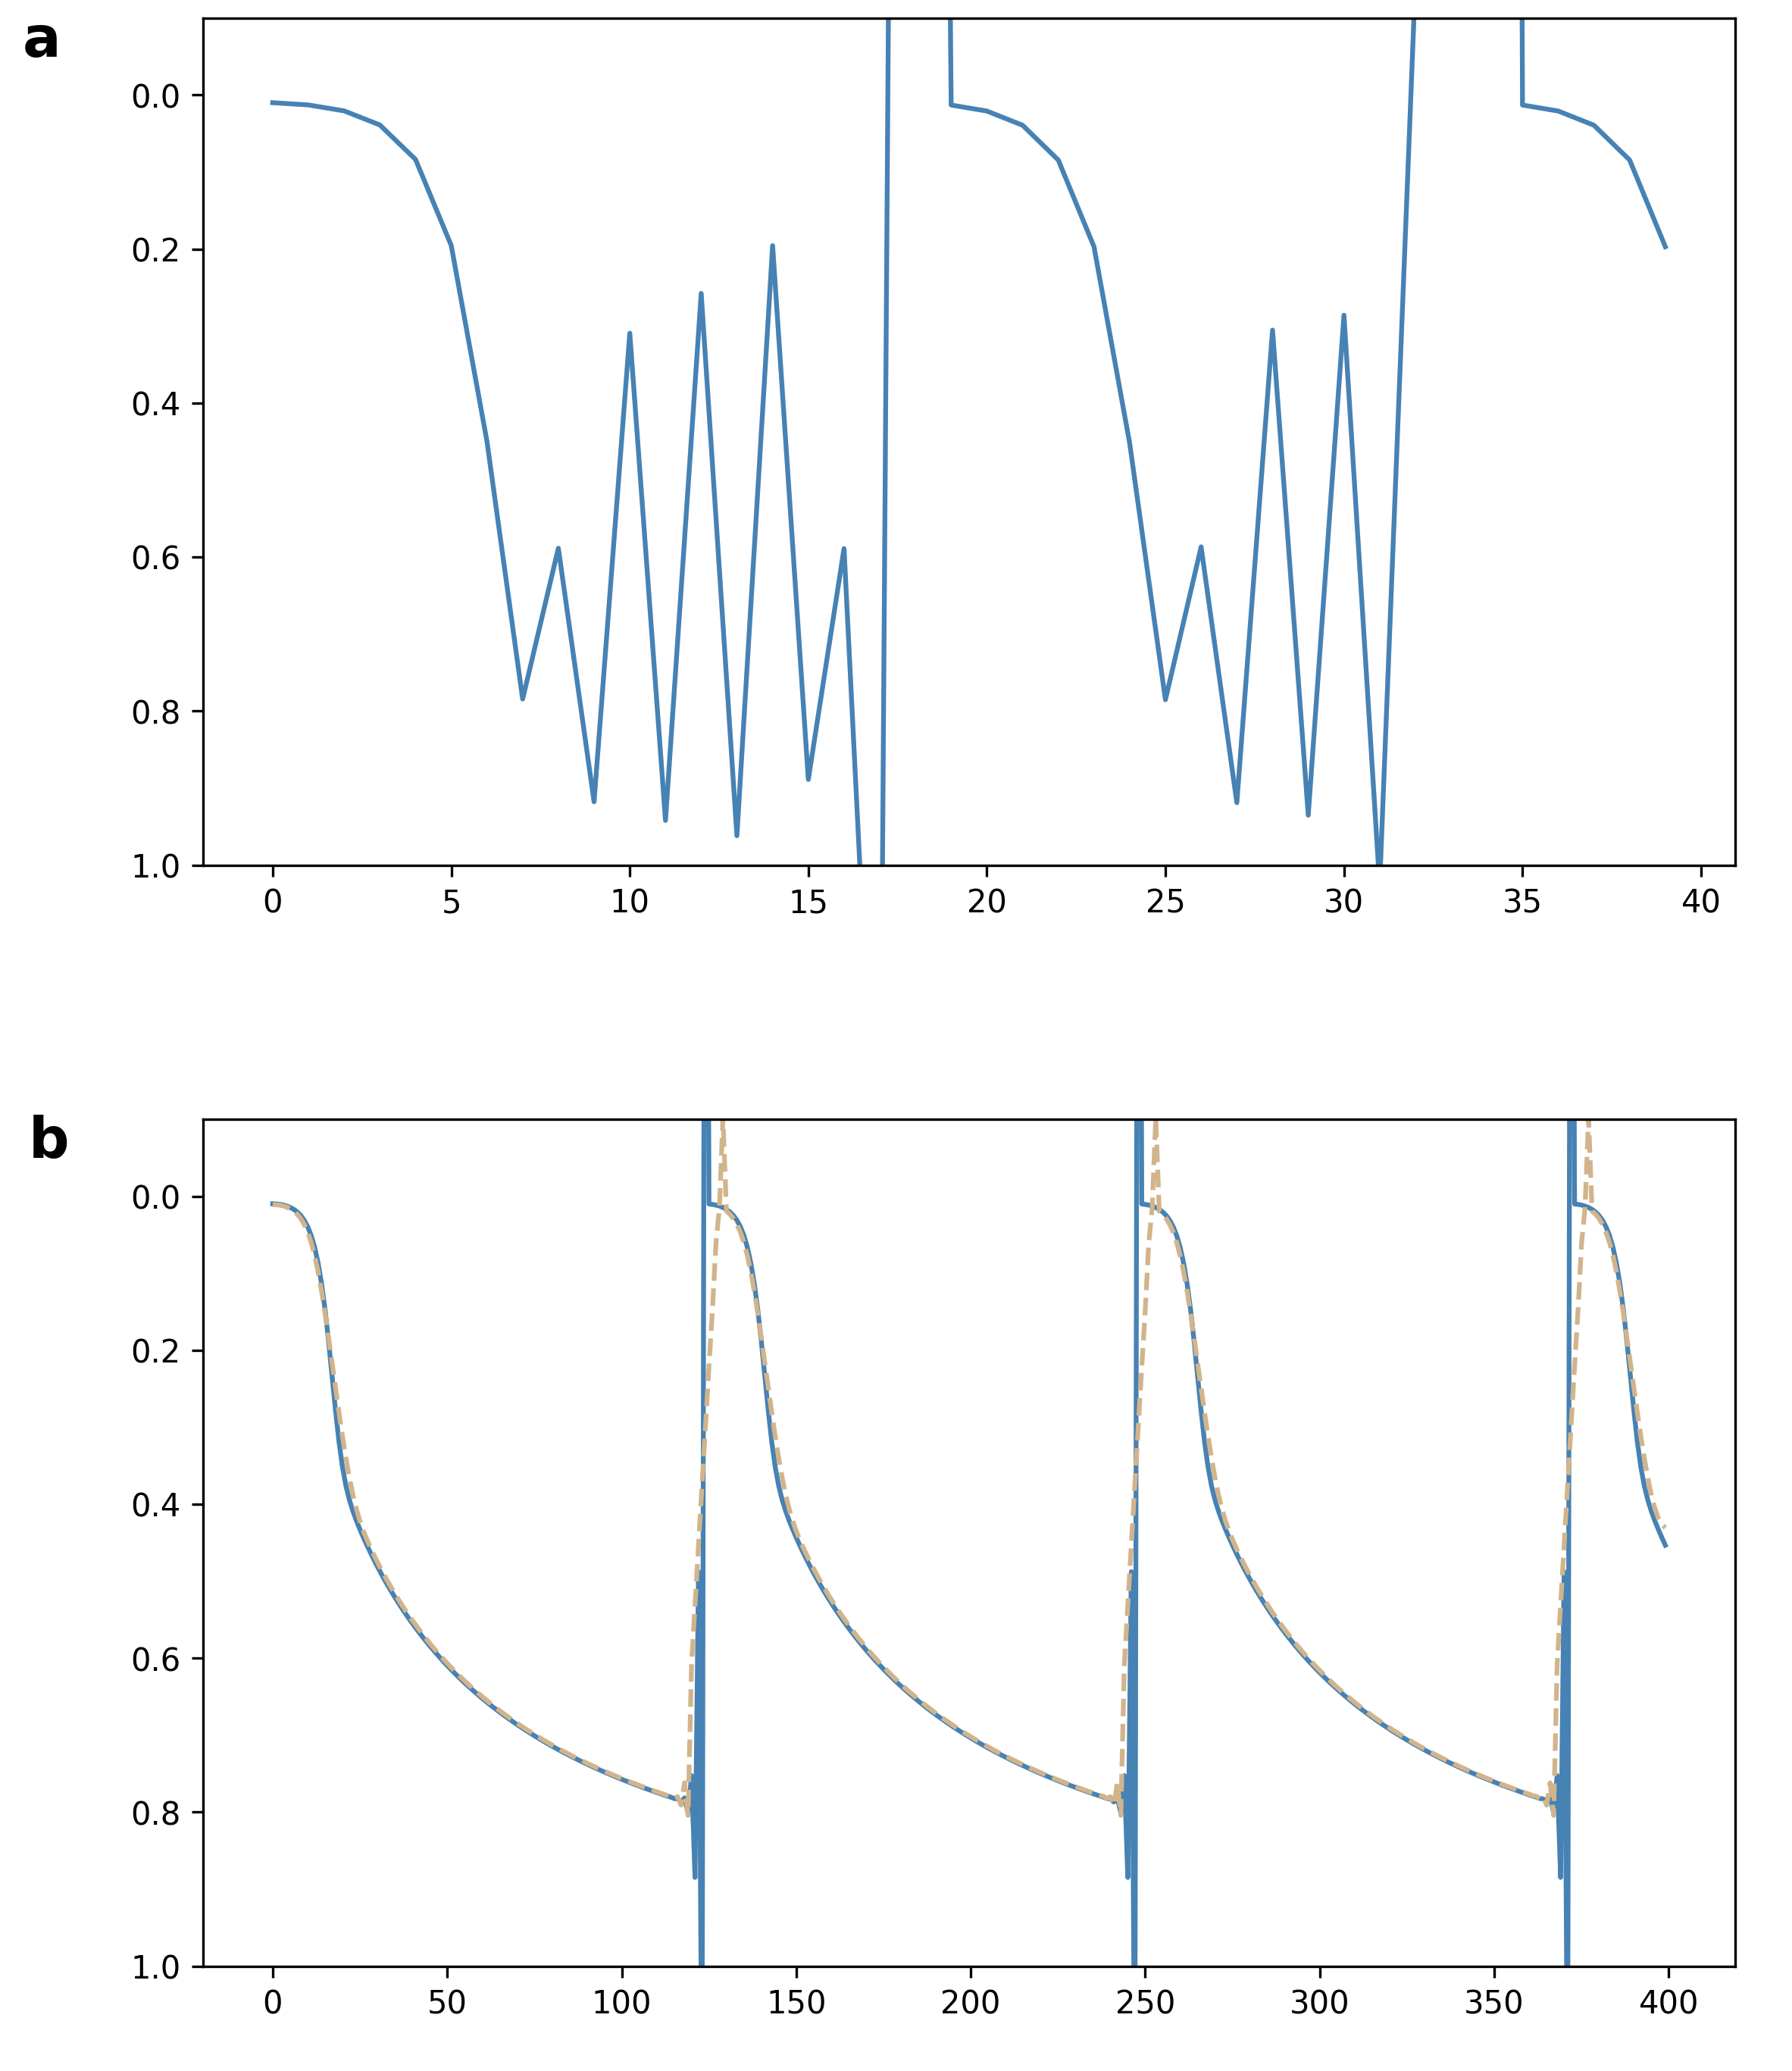
\includegraphics[width=4.25cm]{images/PP-sensitivity.png}

\end{columns}


\end{frame}


%%%%%%%%%%%%%%%%%%%%%%%%


\begin{frame}{\insertsectionnumber{ |} Fundamentals of numerical modelling}


\begin{columns}

\column[c]{4.5cm}

\begin{beamerboxesrounded}[lower=gray,shadow=true]{
\begin{itemize}
\item Often the equations we are trying to solve are differential equations, i.e. they describe a quantity that changes through time
\end{itemize}
\centering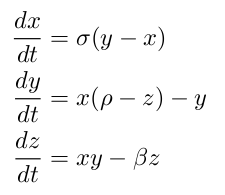
\includegraphics[width=3cm]{images/lorenz_eqs.png}\\
}
\end{beamerboxesrounded}

\column[c]{6.5cm}
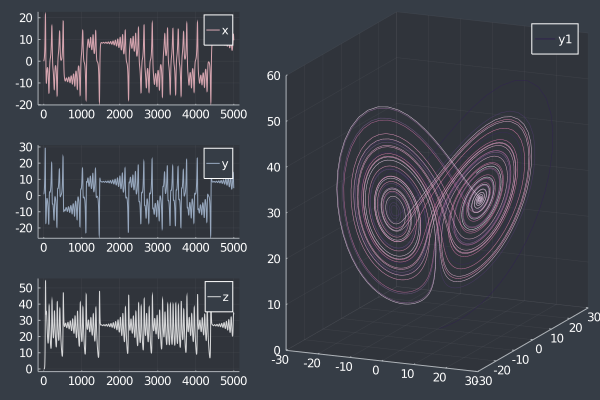
\includegraphics[width=6.5cm]{images/lorenz.png}
%\href{run:mplayer ./images/lorenz_2.gif}{
%\includegraphics[scale=0.25]
%{./images/lorenz_eqs.png}}
\end{columns}
\vspace*{0.5cm}\centering{Lorenz equations (of atmospheric convection)} \\

\end{frame}



%%%%%%%%%%%%%%%%%%%%%%%%


\begin{frame}{\insertsectionnumber{ |} Numerical modelling: epidemics}

A good example of a system that changes through time with no inherently predictable\footnote{actually, for a simple system an analytical solution is possible}  outcome is the spread of an epidemic:

\begin{columns}

\hspace*{1cm}\column[c]{4.5cm}

\vspace*{0.5cm}\begin{beamerboxesrounded}[lower=gray,shadow=true]{

\begin{itemize}
\item We can define differential equations for different components of the susceptible population
\begin{itemize}
\item Susceptible
\item Exposed
\item Infected
\item Recovered
\end{itemize}
\end{itemize}
}
\end{beamerboxesrounded}

\begin{beamerboxesrounded}[lower=gray,shadow=true]{
\centering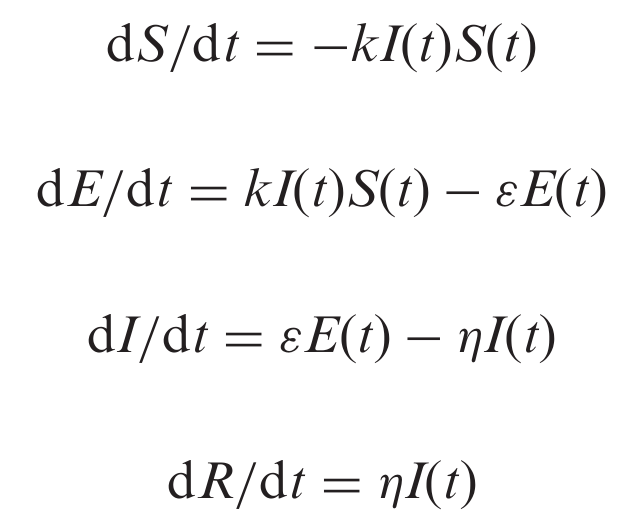
\includegraphics[width=3cm]{images/SEIR_eqs.png}\\

}
\end{beamerboxesrounded}



\hspace*{1cm}\column[c]{3.5cm}
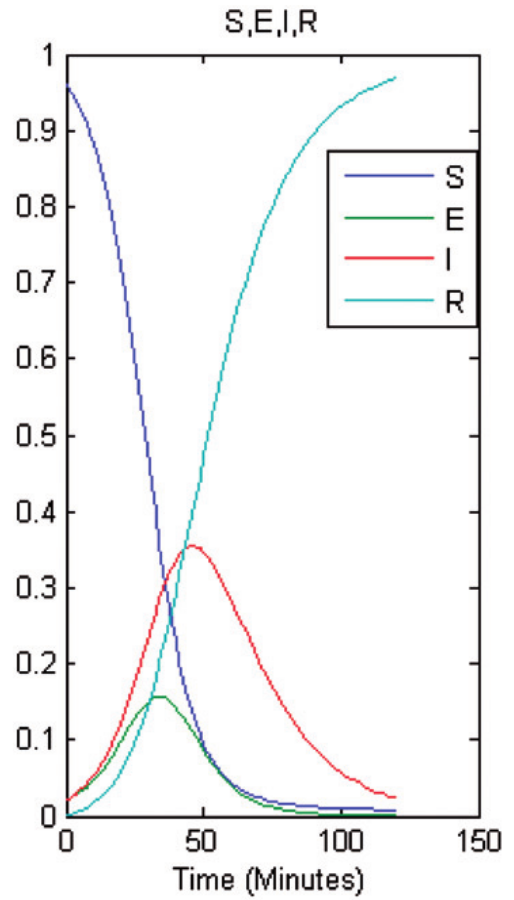
\includegraphics[width=3.5cm]{images/SEIR_plot.png}
%\href{run:mplayer ./images/lorenz_2.gif}{
%\includegraphics[scale=0.25]
%{./images/lorenz_eqs.png}}
\end{columns}

\vspace*{0.5cm}\centering{(Bilge et al., 2012)}\\


\end{frame}



%%%%%%%%%%%%%%%%%%%%%%%%


\begin{frame}{\insertsectionnumber{ |} Numerical modelling: epidemics}


\hspace*{-0.75cm}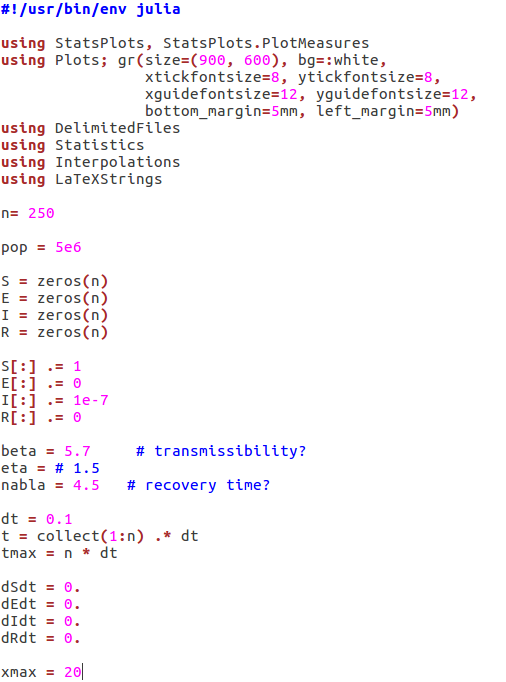
\includegraphics[height=6.75cm]{images/epi1D_1.png}
\hspace*{-0.1cm}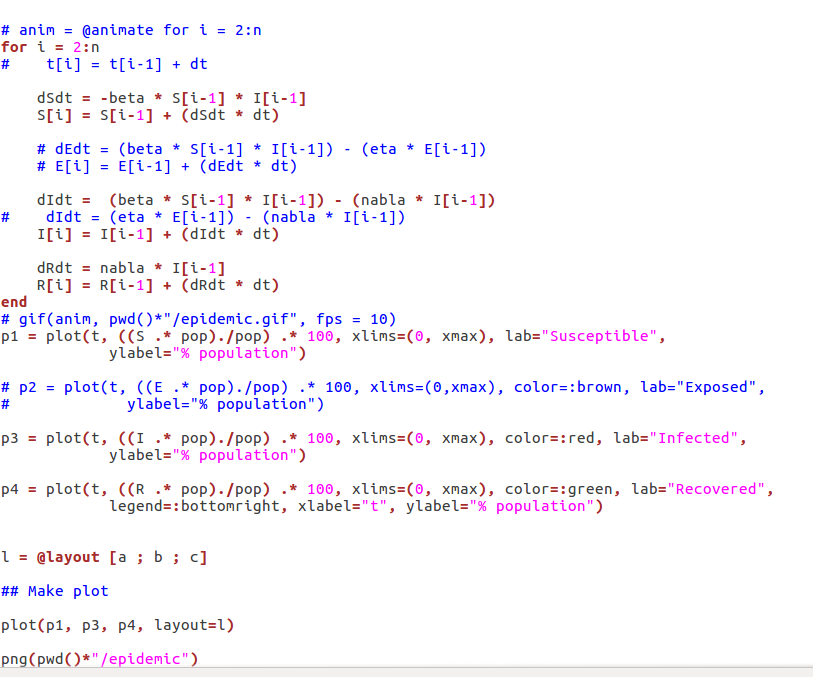
\includegraphics[height=6.75cm]{images/epi1D_2.png}


\end{frame}



%%%%%%%%%%%%%%%%%%%%%%%%


\begin{frame}{\insertsectionnumber{ |} Numerical modelling: epidemics}


\centering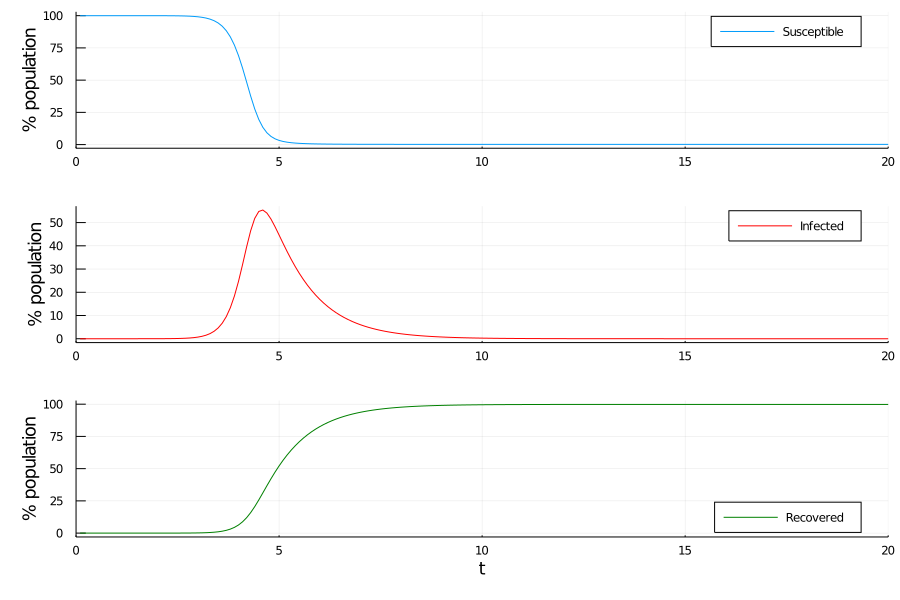
\includegraphics[width=9cm]{images/epidemic.png}\\


\end{frame}




%%%%%%%%%%%%%%%%%%%%%%%%


\begin{frame}{\insertsectionnumber{ |} Numerical modelling: epidemics}

\begin{beamerboxesrounded}[lower=gray,shadow=true]{

\begin{itemize}
\item Simple 1D system treats entire population as a bulk quantity
\item Makes \emph{lots} of simplifying assumptions:
\begin{itemize}
\item Entirety of population are equally susceptible
\item `Perfect' transmission occurs
\item Recovery is just a matter of (uniform) time
\item Full immunity follows
\end{itemize}
\item Good for understanding evolution of a simple system, but not very realistic
\end{itemize}

}

\end{beamerboxesrounded}

\vspace*{1cm}\begin{beamerboxesrounded}[lower=gray,shadow=true]{

Is it realistic to simulate epidemic evolution as a diffusive system?

\begin{itemize}
\item A `better' approach might be to consider transmission in spatial (as well as temporal) domain
\item We could also introduce some randomness to allow for individual differences / chance occurrence in transmission \& recovery
\item What if people die?
\item What if people get reinfected?
\end{itemize}
}

\end{beamerboxesrounded}
\end{frame}




%%%%%%%%%%%%%%%%%%%%%%%%


\begin{frame}{\insertsectionnumber{ |} Numerical modelling: epidemics}

\begin{columns}
\hspace*{-0.25cm}\column[c]{4cm}




\begin{beamerboxesrounded}[lower=gray,shadow=true]{

\begin{itemize}
\item Cellular automata are non-physical statistical models that are useful for spatial problems
\item Instead of percolation or diffusion equations, these are rule-based models
\item They treat evolution of each discrete cell as dependent on the properties of neighbouring cells
\item Allows for very complex scenarios, based primarily on a probabilistic rather than deterministic approach
\end{itemize}

}

\end{beamerboxesrounded}


\hspace*{-0.65cm}\column[c]{7.5cm}

\centering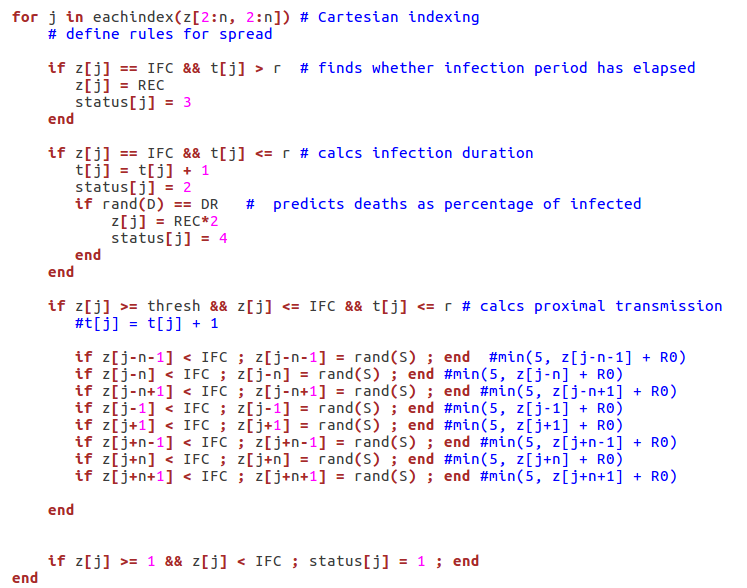
\includegraphics[width=7.5cm]{images/epi2D_1.png}\\

\end{columns}

\end{frame}

%%%%%%%%%%%%%%%%%%%%%%%% END CONTENT %%%%%%%%%%%%%%%%%%%%%%
